\documentclass[12pt,a4paper]{article}
\usepackage{ctex}
\title{神经网络语言模型实验报告}
\author{}

\usepackage{hyperref}
\hypersetup{colorlinks=true, linkcolor=blue, anchorcolor=green, citecolor=green}
\usepackage{bm}
\usepackage{amssymb, amsmath, amsthm}
\usepackage{graphicx}
\usepackage{float}
\usepackage{booktabs}
\usepackage{multirow}
\usepackage{subcaption}
\usepackage{listings}
\usepackage{xcolor}
\usepackage{enumitem}

\lstset{
    language=Python,
    basicstyle=\ttfamily\small,
    keywordstyle=\color{blue},
    commentstyle=\color{gray},
    stringstyle=\color{red},
    breaklines=true,
    frame=single,
    numbers=left,
    numberstyle=\tiny\color{gray}
}

\begin{document}

\begin{titlepage}
    \centering
    \vspace*{1cm}
    
\includegraphics[width=0.6\textwidth]{ucas_logo.pdf}
    \vspace{1cm}

    {\Huge\bfseries 深度学习作业7\par}
    \vspace{1cm}
    {\LARGE 神经网络语言模型实验\par}
    \vspace{3cm}

    \begin{tabular}{rl}
        {\kaishu\Large 成员：} & {\kaishu\Large \underline{\makebox[6cm]{202528014629014 刘浩}}} \\[0.8cm]
         & {\kaishu\Large \underline{\makebox[6cm]{202528014629012 雷夕入}}} \\[0.8cm]
         & {\kaishu\Large \underline{\makebox[6cm]{202528014629015 刘宇坤}}} \\[0.8cm]
        {\kaishu\Large 院所：} & {\kaishu\Large \underline{\makebox[6cm]{人工智能学院}}} \\[0.8cm]
    \end{tabular}

    \vfill

    {\large \today\par}
\end{titlepage}

\newpage
\tableofcontents
\newpage

\section{实验目的}

本实验旨在深入理解循环神经网络语言模型的基本原理与实现方法，通过在Penn Treebank数据集上训练不同规模的LSTM语言模型，掌握序列建模的核心技术。实验要求模型在测试集上的困惑度（Perplexity）低于80，同时需要对比分析小型、中型和大型三种模型配置的性能差异，理解模型容量、正则化强度与泛化性能之间的关系。

\section{实验原理}

\subsection{循环神经网络与LSTM}

语言建模的目标是学习一个概率分布$P(w_1, w_2, \ldots, w_T)$，通过链式法则将其分解为条件概率的连乘：
\begin{equation}
P(w_1, w_2, \ldots, w_T) = \prod_{t=1}^{T}P(w_t | w_1, \ldots, w_{t-1})
\end{equation}

LSTM通过门控机制解决了标准RNN的梯度消失问题，其核心计算过程为：
\begin{align}
f_t &= \sigma(W_f[h_{t-1}, x_t] + b_f) \\
i_t &= \sigma(W_i[h_{t-1}, x_t] + b_i) \\
\tilde{c}_t &= \tanh(W_c[h_{t-1}, x_t] + b_c) \\
c_t &= f_t \odot c_{t-1} + i_t \odot \tilde{c}_t \\
o_t &= \sigma(W_o[h_{t-1}, x_t] + b_o) \\
h_t &= o_t \odot \tanh(c_t)
\end{align}
其中$f_t$、$i_t$、$o_t$分别为遗忘门、输入门和输出门，$c_t$为细胞状态，$\odot$表示逐元素乘法。

\subsection{困惑度}

困惑度是评价语言模型质量的标准指标，定义为测试集上交叉熵损失的指数：
\begin{equation}
\text{PPL} = \exp\left(-\frac{1}{T}\sum_{t=1}^{T}\log P(w_t | w_{<t})\right)
\end{equation}
直观地，困惑度可以理解为模型在每个位置上的平均候选词数量。困惑度越低，说明模型对语言的建模越精确。

\subsection{正则化技术}

为防止过拟合，实验采用多种正则化手段：Dropout应用于LSTM层之间和词嵌入层，随机丢弃一定比例的神经元；权重绑定（weight tying）将输入词嵌入矩阵和输出softmax层的权重共享，既减少了参数量又起到了正则化效果。此外，通过时间维度的反向传播截断（Truncated BPTT）限制梯度传播的时间步长，平衡计算效率与长距离依赖建模。

\section{数据集分析}

Penn Treebank（PTB）是自然语言处理领域最经典的基准数据集之一，经过标准预处理后包含约929K训练词、73K验证词和82K测试词，词表大小为10000。数据集源自华尔街日报的新闻文本，预处理过程中将所有词转为小写，数字替换为特殊标记，低频词替换为\texttt{<unk>}标记。

PTB数据集的规模相对较小，这使得模型容易过拟合，因此成为检验正则化技术有效性的理想测试平台。数据集中的文本涵盖金融、政治、体育等多个领域，词汇使用较为正式和多样，对语言模型的建模能力提出了全面的要求。

\section{模型设计与实现}

本实验设计了三种不同规模的LSTM语言模型进行对比：

\begin{table}[H]
\centering
\caption{三种模型配置对比}
\label{tab:config}
\resizebox{\textwidth}{!}{
\begin{tabular}{lccccc}
\toprule
\textbf{模型} & \textbf{层数} & \textbf{隐藏维度} & \textbf{嵌入维度} & \textbf{Dropout} & \textbf{训练时间/epoch} \\
\midrule
Small  & 2 & 200  & 200  & 0.2  & $\sim$7.7s \\
Medium & 2 & 650  & 650  & 0.5  & $\sim$15.5s \\
Large  & 2 & 1500 & 1500 & 0.65 & $\sim$41.1s \\
\bottomrule
\end{tabular}
}
\end{table}

三种模型均采用权重绑定策略，将输入嵌入层和输出投影层的权重矩阵共享。随着模型容量的增大，Dropout率也相应提高（从0.2到0.65），以平衡表达能力与过拟合风险。

训练采用SGD优化器，初始学习率为20。当验证集困惑度不再下降时，学习率除以4。BPTT截断长度设为35，梯度裁剪阈值为0.25，防止梯度爆炸。batch size设为20。

\section{实验结果与分析}

\subsection{训练困惑度}

图\ref{fig:train_ppl}展示了三种模型在训练集上困惑度的变化。Large模型由于容量最大，训练困惑度下降最快，最终降至40.47；Medium模型收敛至44.91；Small模型受限于表达能力，最终训练PPL为71.64。三者的差距反映了模型容量对训练集拟合能力的直接影响。

\begin{figure}[H]
\centering
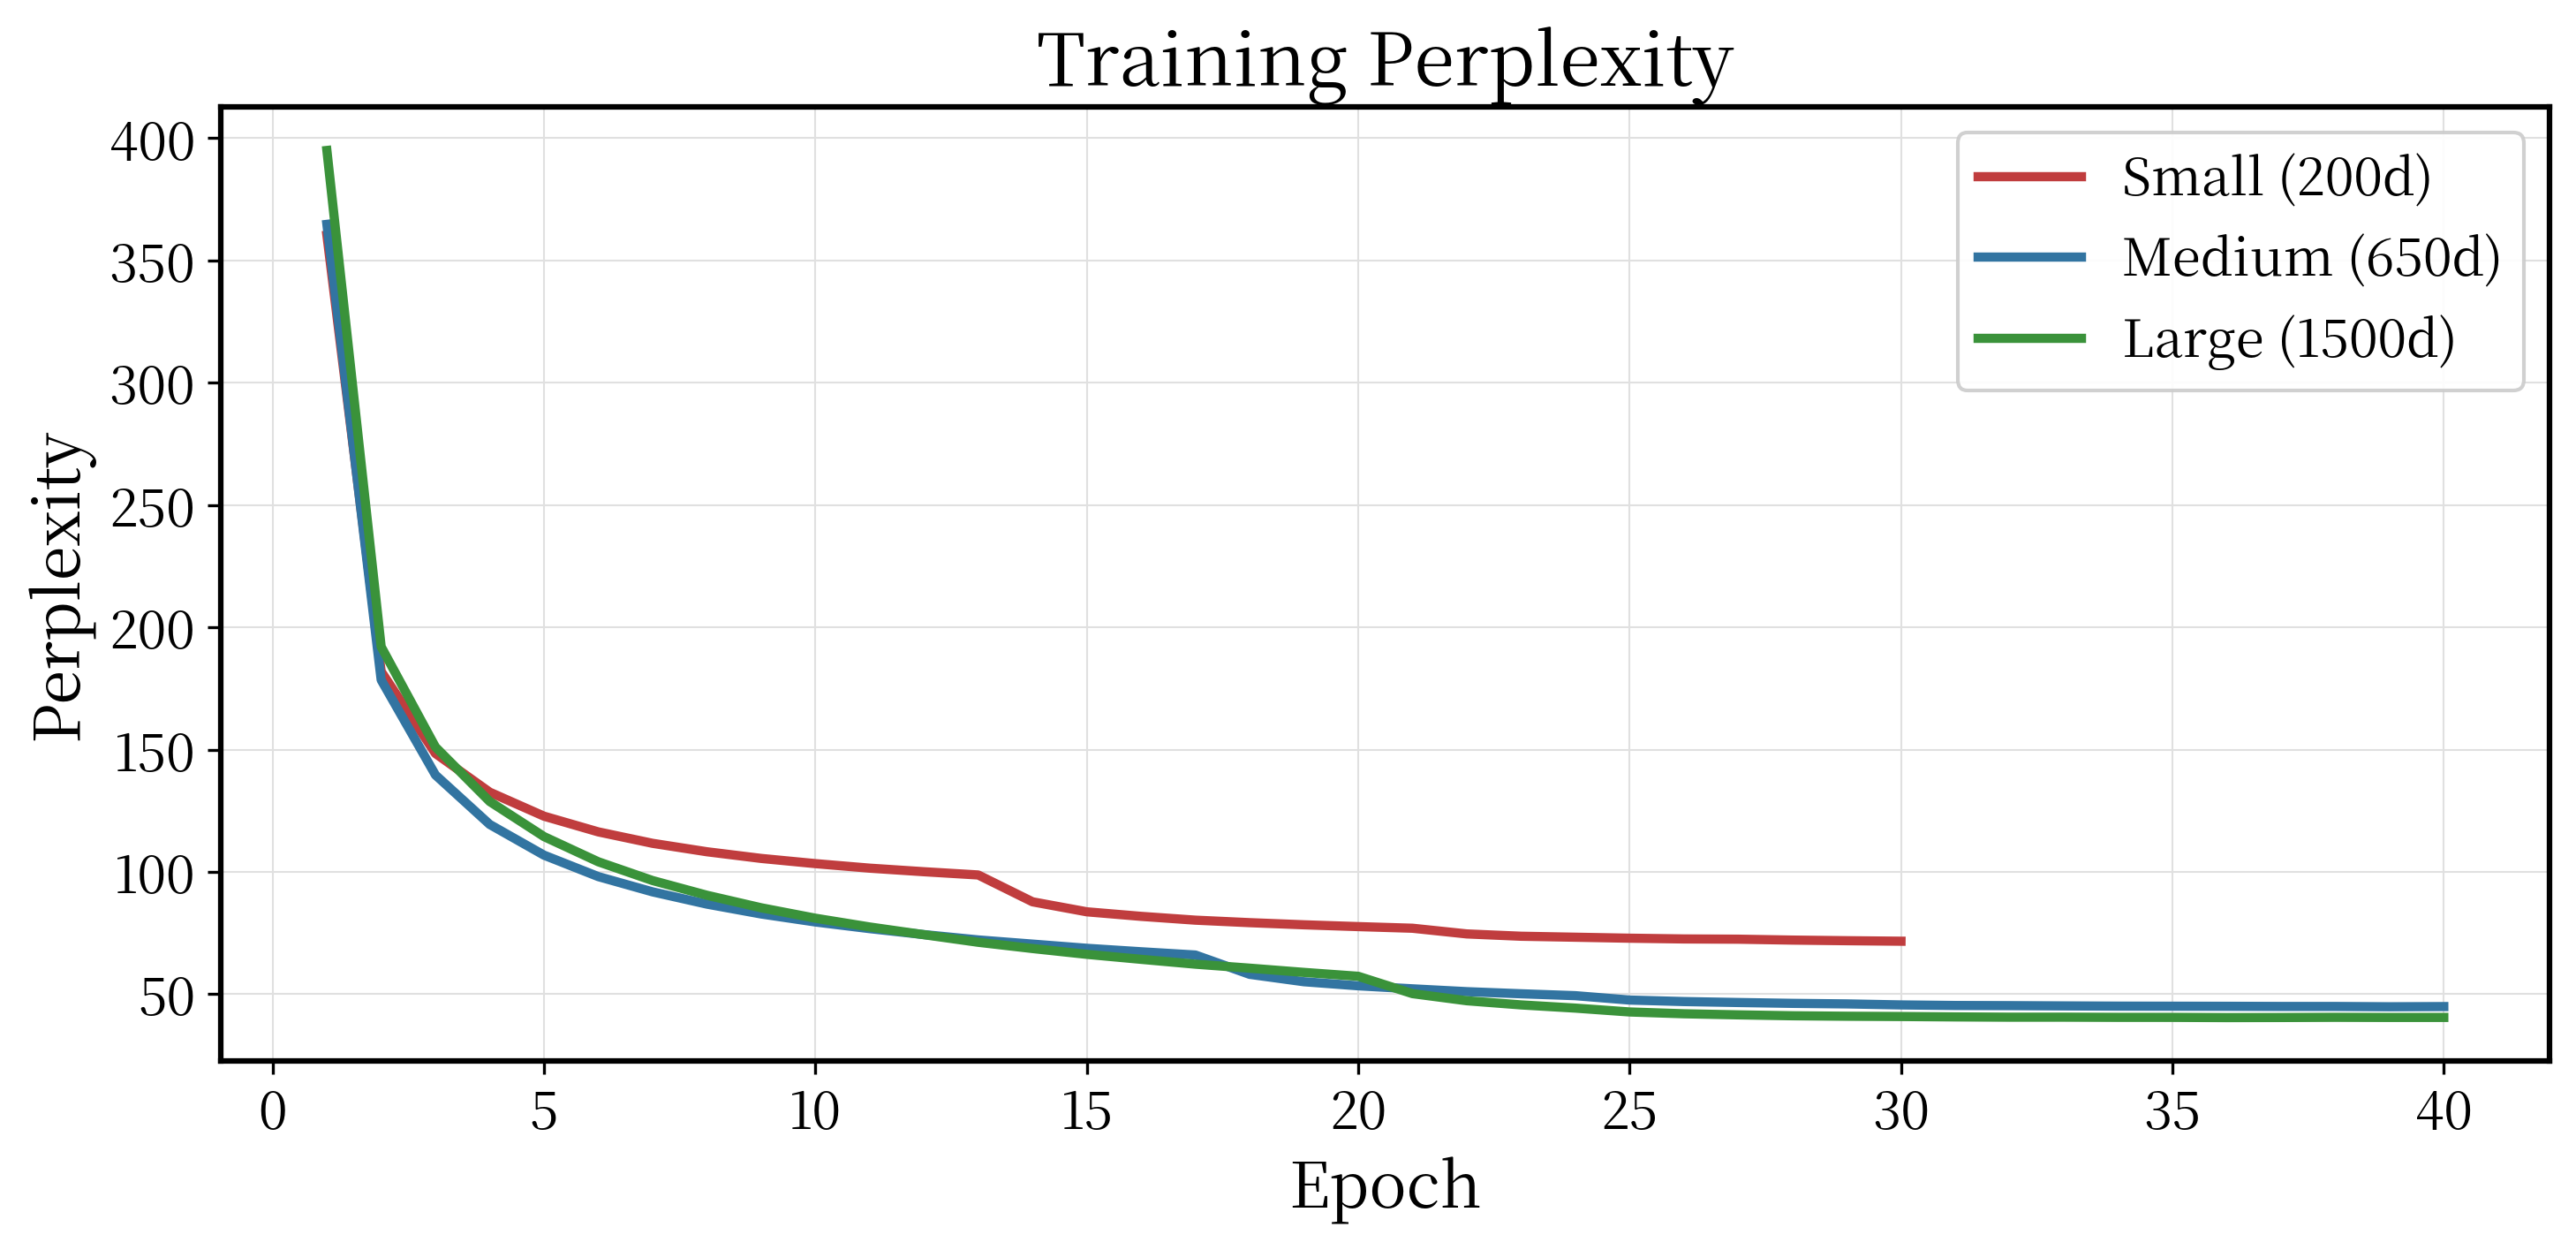
\includegraphics[width=0.8\textwidth]{figs/fig01_train_ppl.png}
\caption{训练集困惑度变化曲线}
\label{fig:train_ppl}
\end{figure}

\subsection{验证困惑度}

图\ref{fig:valid_ppl}展示了验证集上的困惑度变化，这是模型选择和学习率衰减的关键依据。Large模型在验证集上最终达到PPL=75.70，Medium模型为79.23，Small模型为92.00。值得注意的是，Large模型在训练集上的优势（PPL相差26.4）在验证集上大幅缩小（PPL仅相差3.5），这说明更大的模型容量主要被用于“记忆”训练数据的细节模式，而非学到更具泛化性的语言规律。

\begin{figure}[H]
\centering
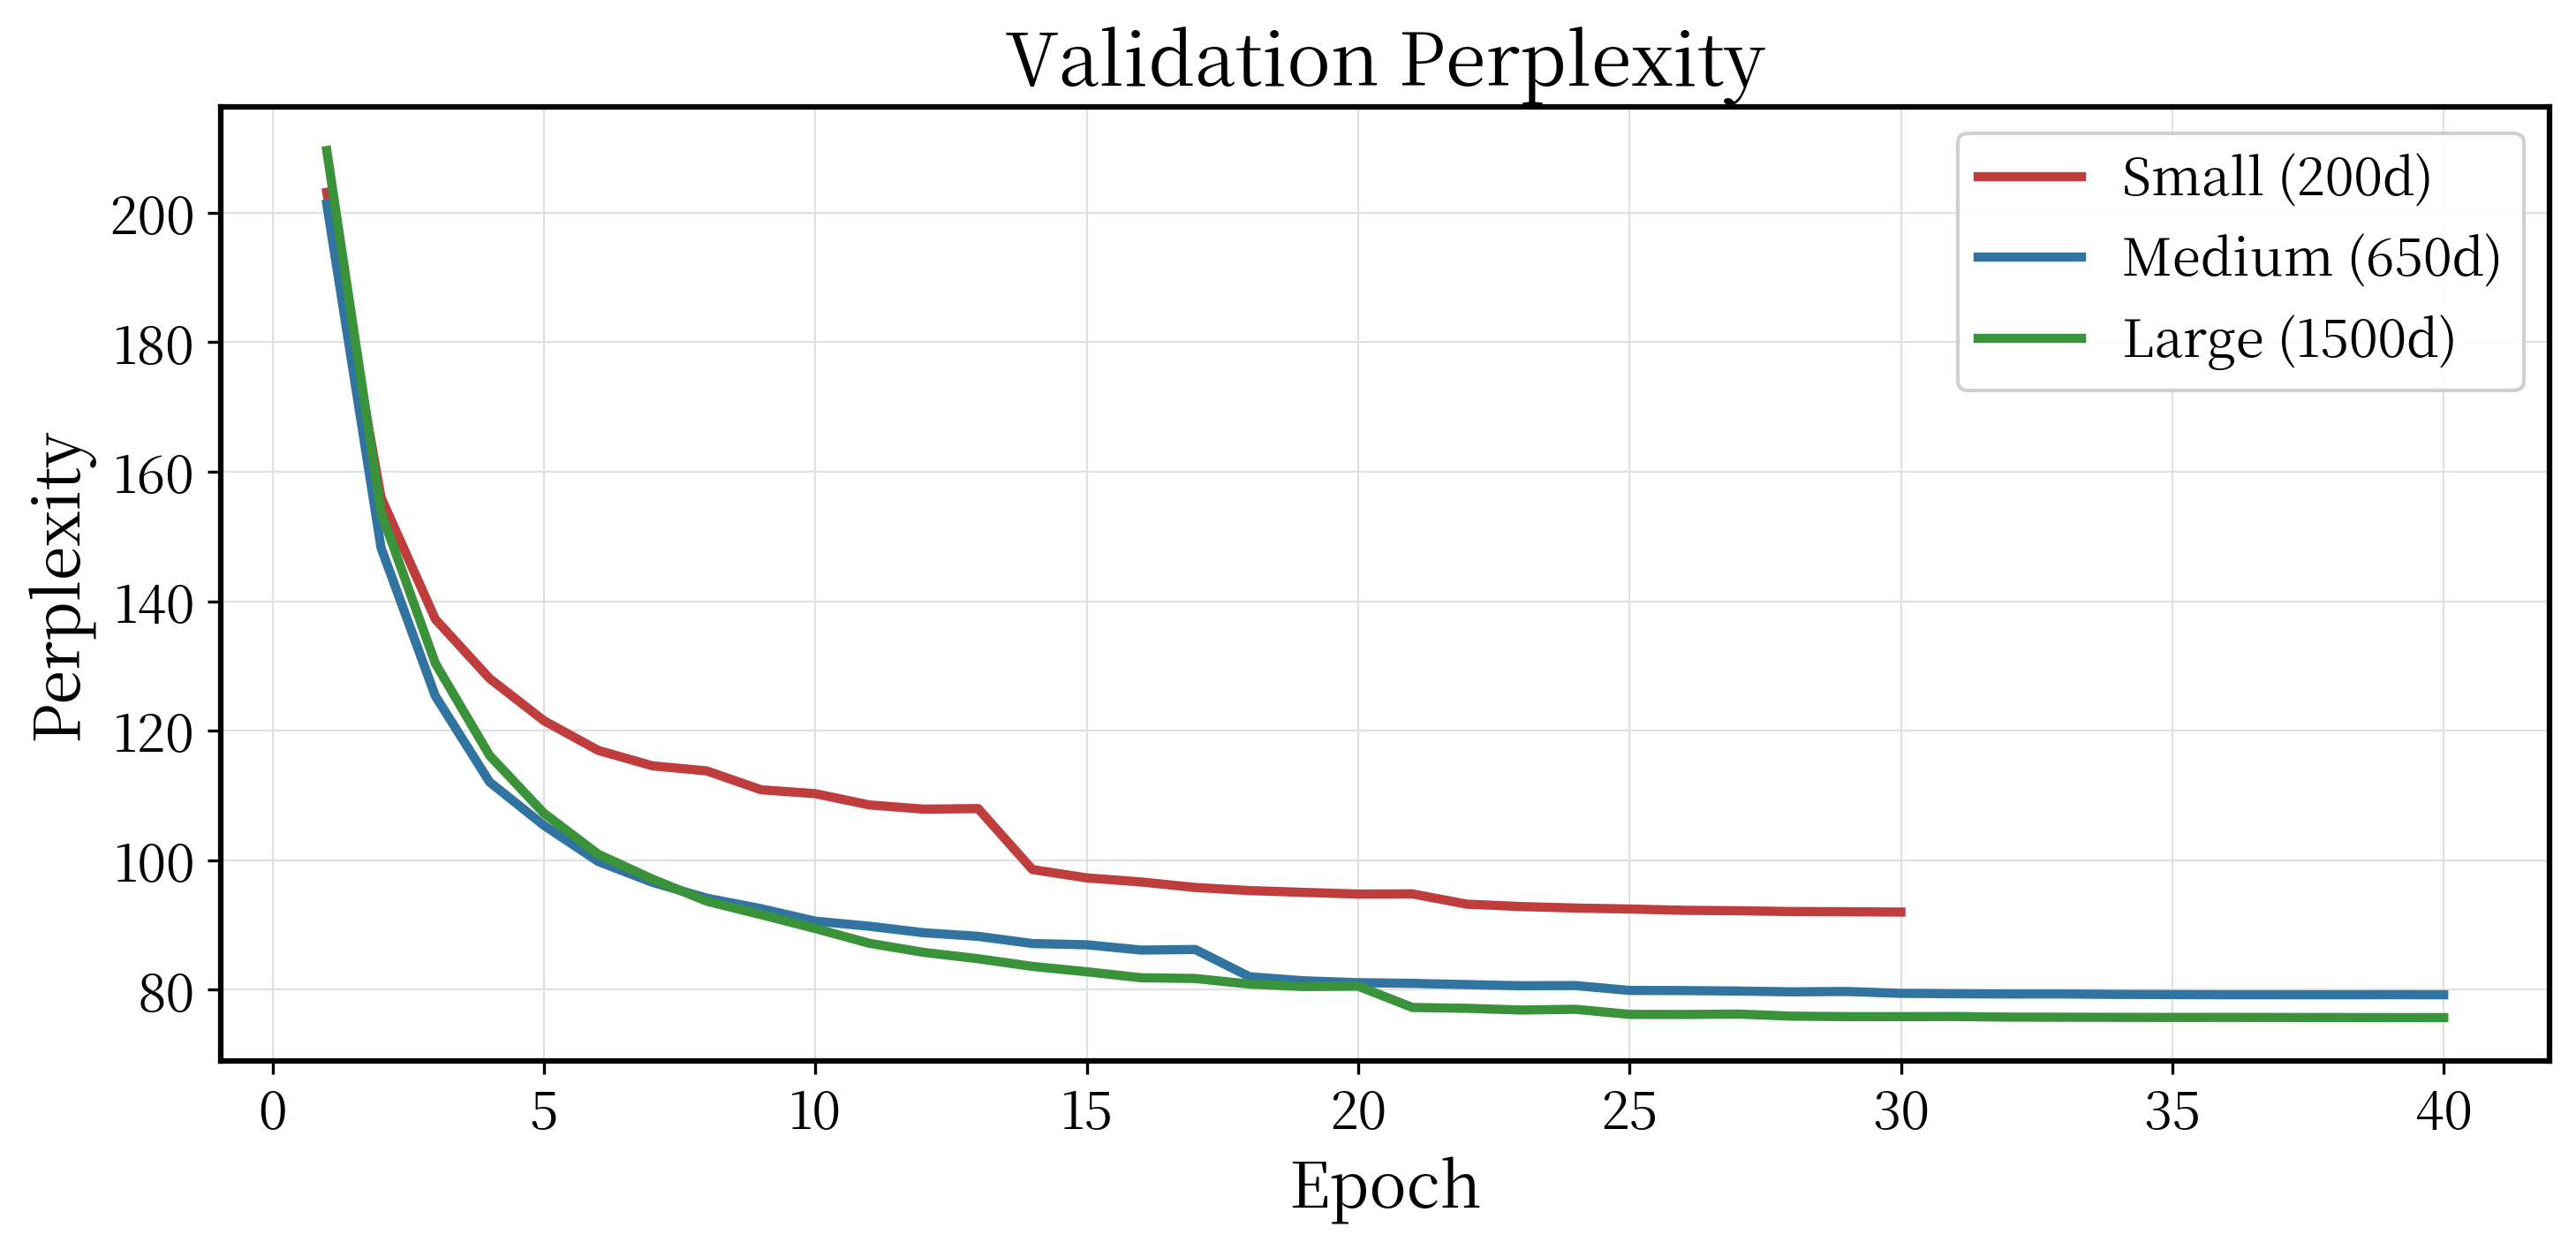
\includegraphics[width=0.8\textwidth]{figs/fig02_valid_ppl.png}
\caption{验证集困惑度变化曲线}
\label{fig:valid_ppl}
\end{figure}

\subsection{学习率与测试结果}

图\ref{fig:lr}展示了学习率的衰减过程。可以观察到三种模型的学习率衰减时机不同：Small模型在第14个epoch首次衰减，Medium在第18个epoch，Large在第21个epoch。更大的模型需要更多epoch才达到验证性能的瓶颈，这与其更复杂的loss surface和更慢的收敛特性一致。每次衰减后，验证困惑度都出现明显的阶梯式下降。

\begin{figure}[H]
\centering
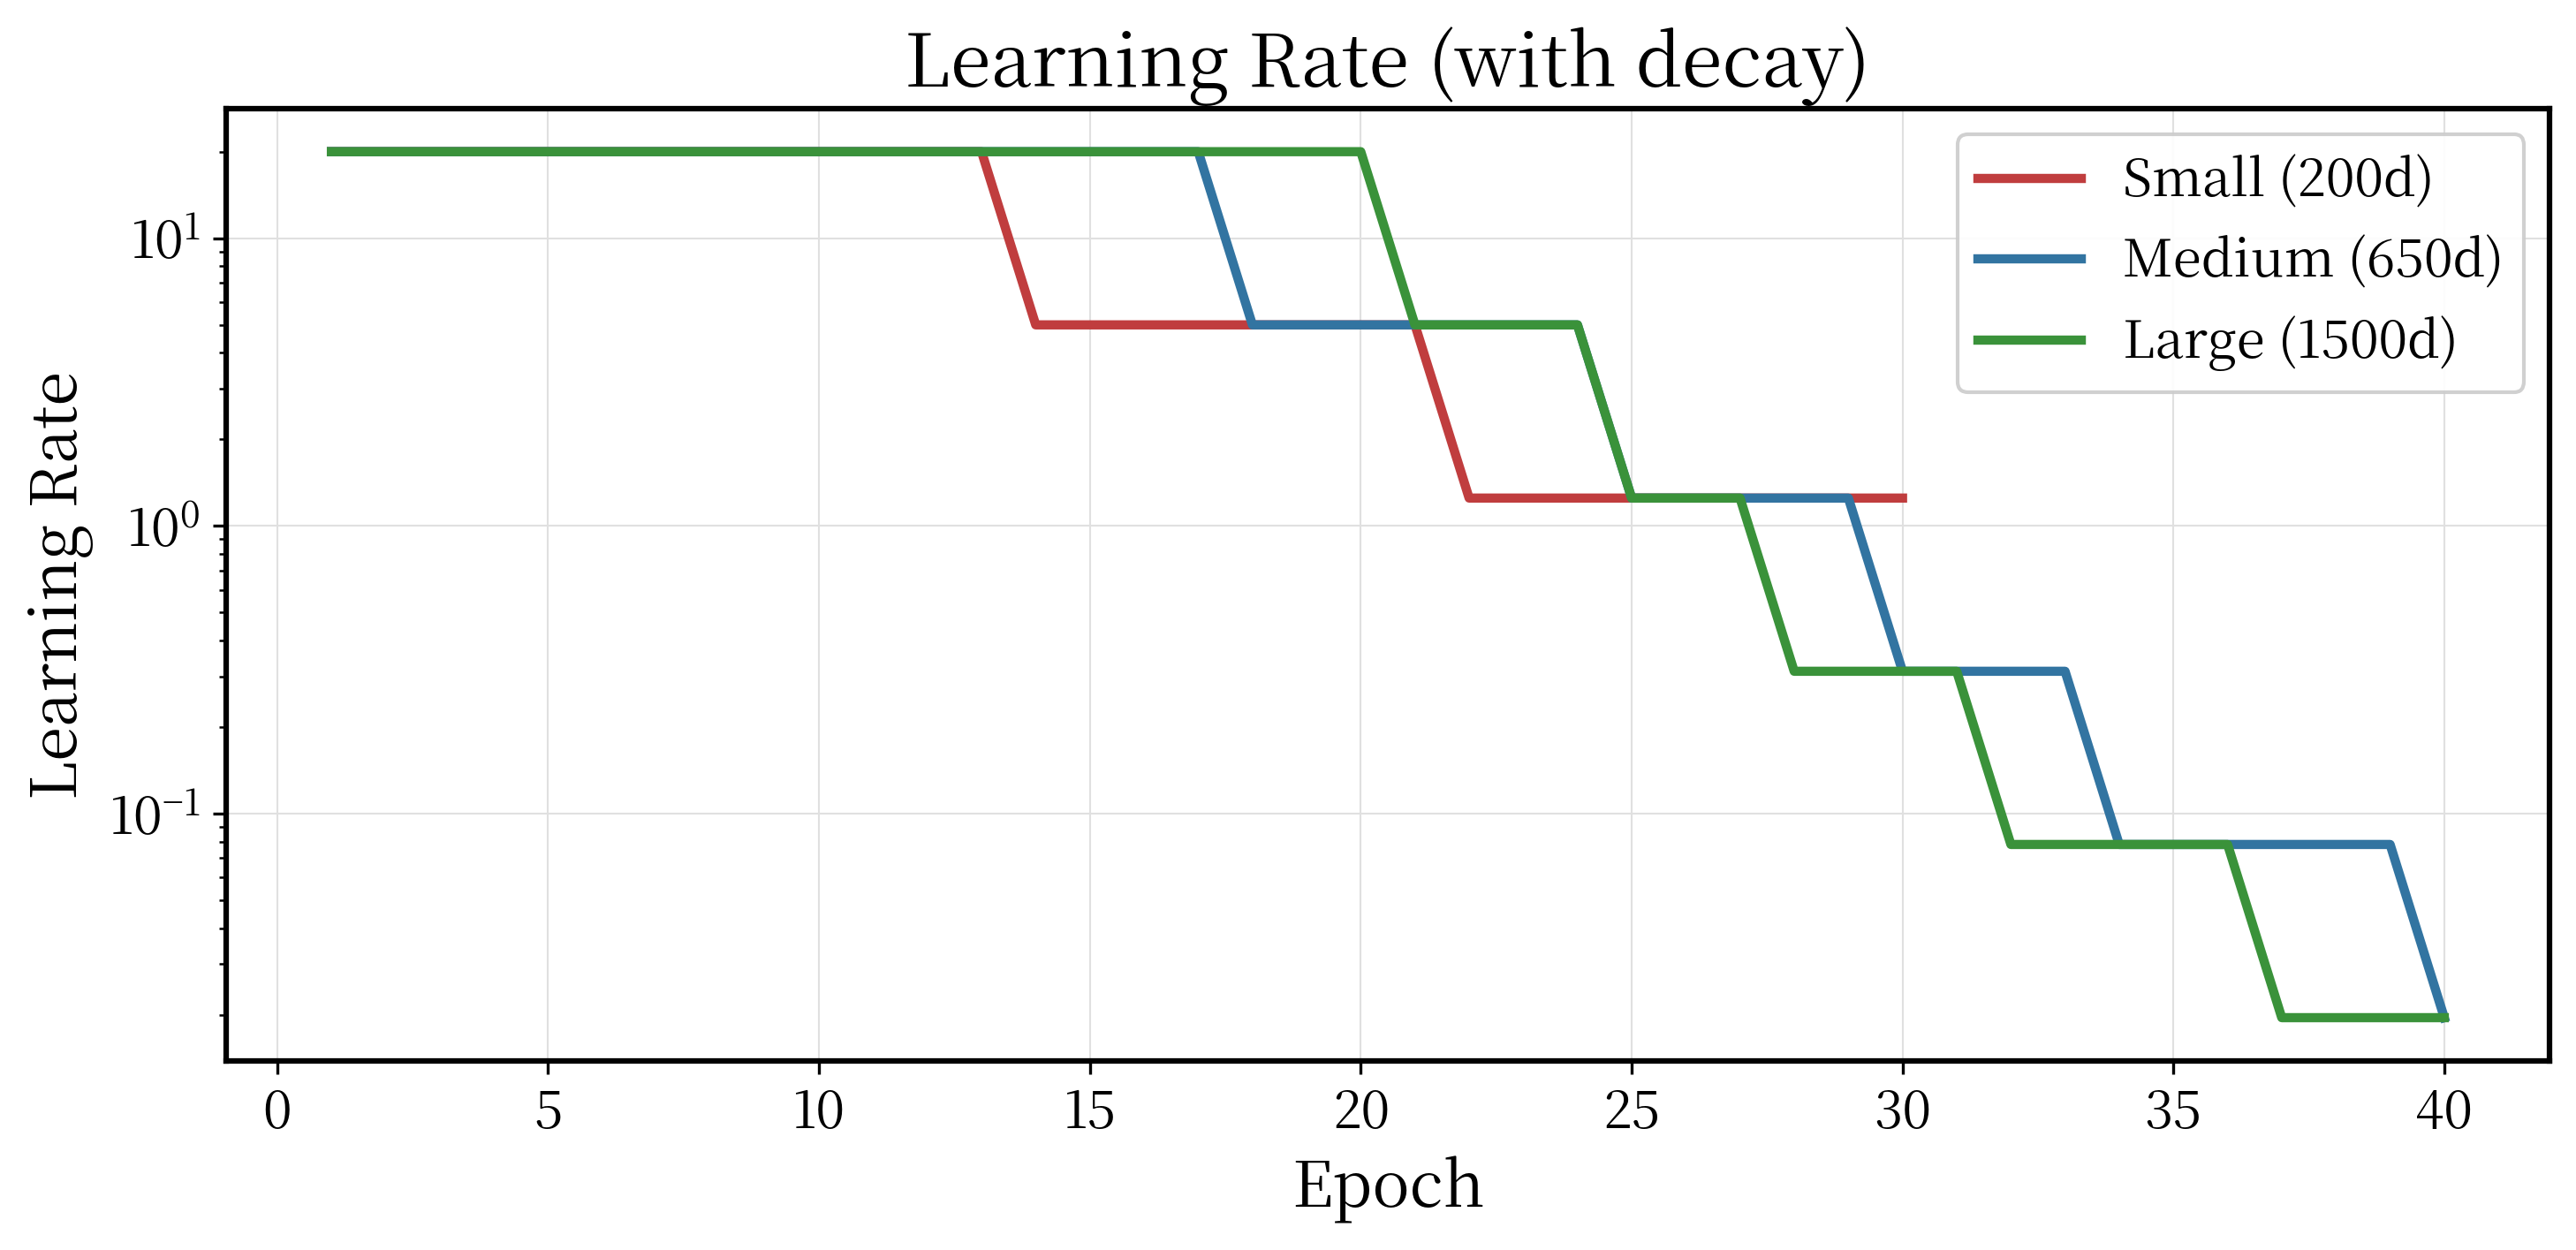
\includegraphics[width=0.8\textwidth]{figs/fig03_lr.png}
\caption{学习率变化曲线}
\label{fig:lr}
\end{figure}

\begin{table}[H]
\centering
\caption{模型最终性能对比}
\label{tab:result}
\resizebox{0.85\textwidth}{!}{
\begin{tabular}{lcccc}
\toprule
\textbf{模型} & \textbf{训练PPL} & \textbf{验证PPL} & \textbf{测试PPL} & \textbf{是否达标} \\
\midrule
Small  & 71.64 & 92.00 & 88.30 & 否 \\
Medium & 44.91 & 79.23 & \textbf{75.92} & 是 \\
Large  & 40.47 & 75.70 & \textbf{72.48} & 是 \\
\bottomrule
\end{tabular}
}
\end{table}

图\ref{fig:test_ppl}展示了最终测试集上的困惑度对比。Medium模型（PPL=75.92）和Large模型（PPL=72.48）均成功达到了PPL低于80的实验目标。Small模型测试PPL=88.30，未能达标，但其训练效率最高（7.7秒/epoch），适合作为快速原型验证使用。

\begin{figure}[H]
\centering
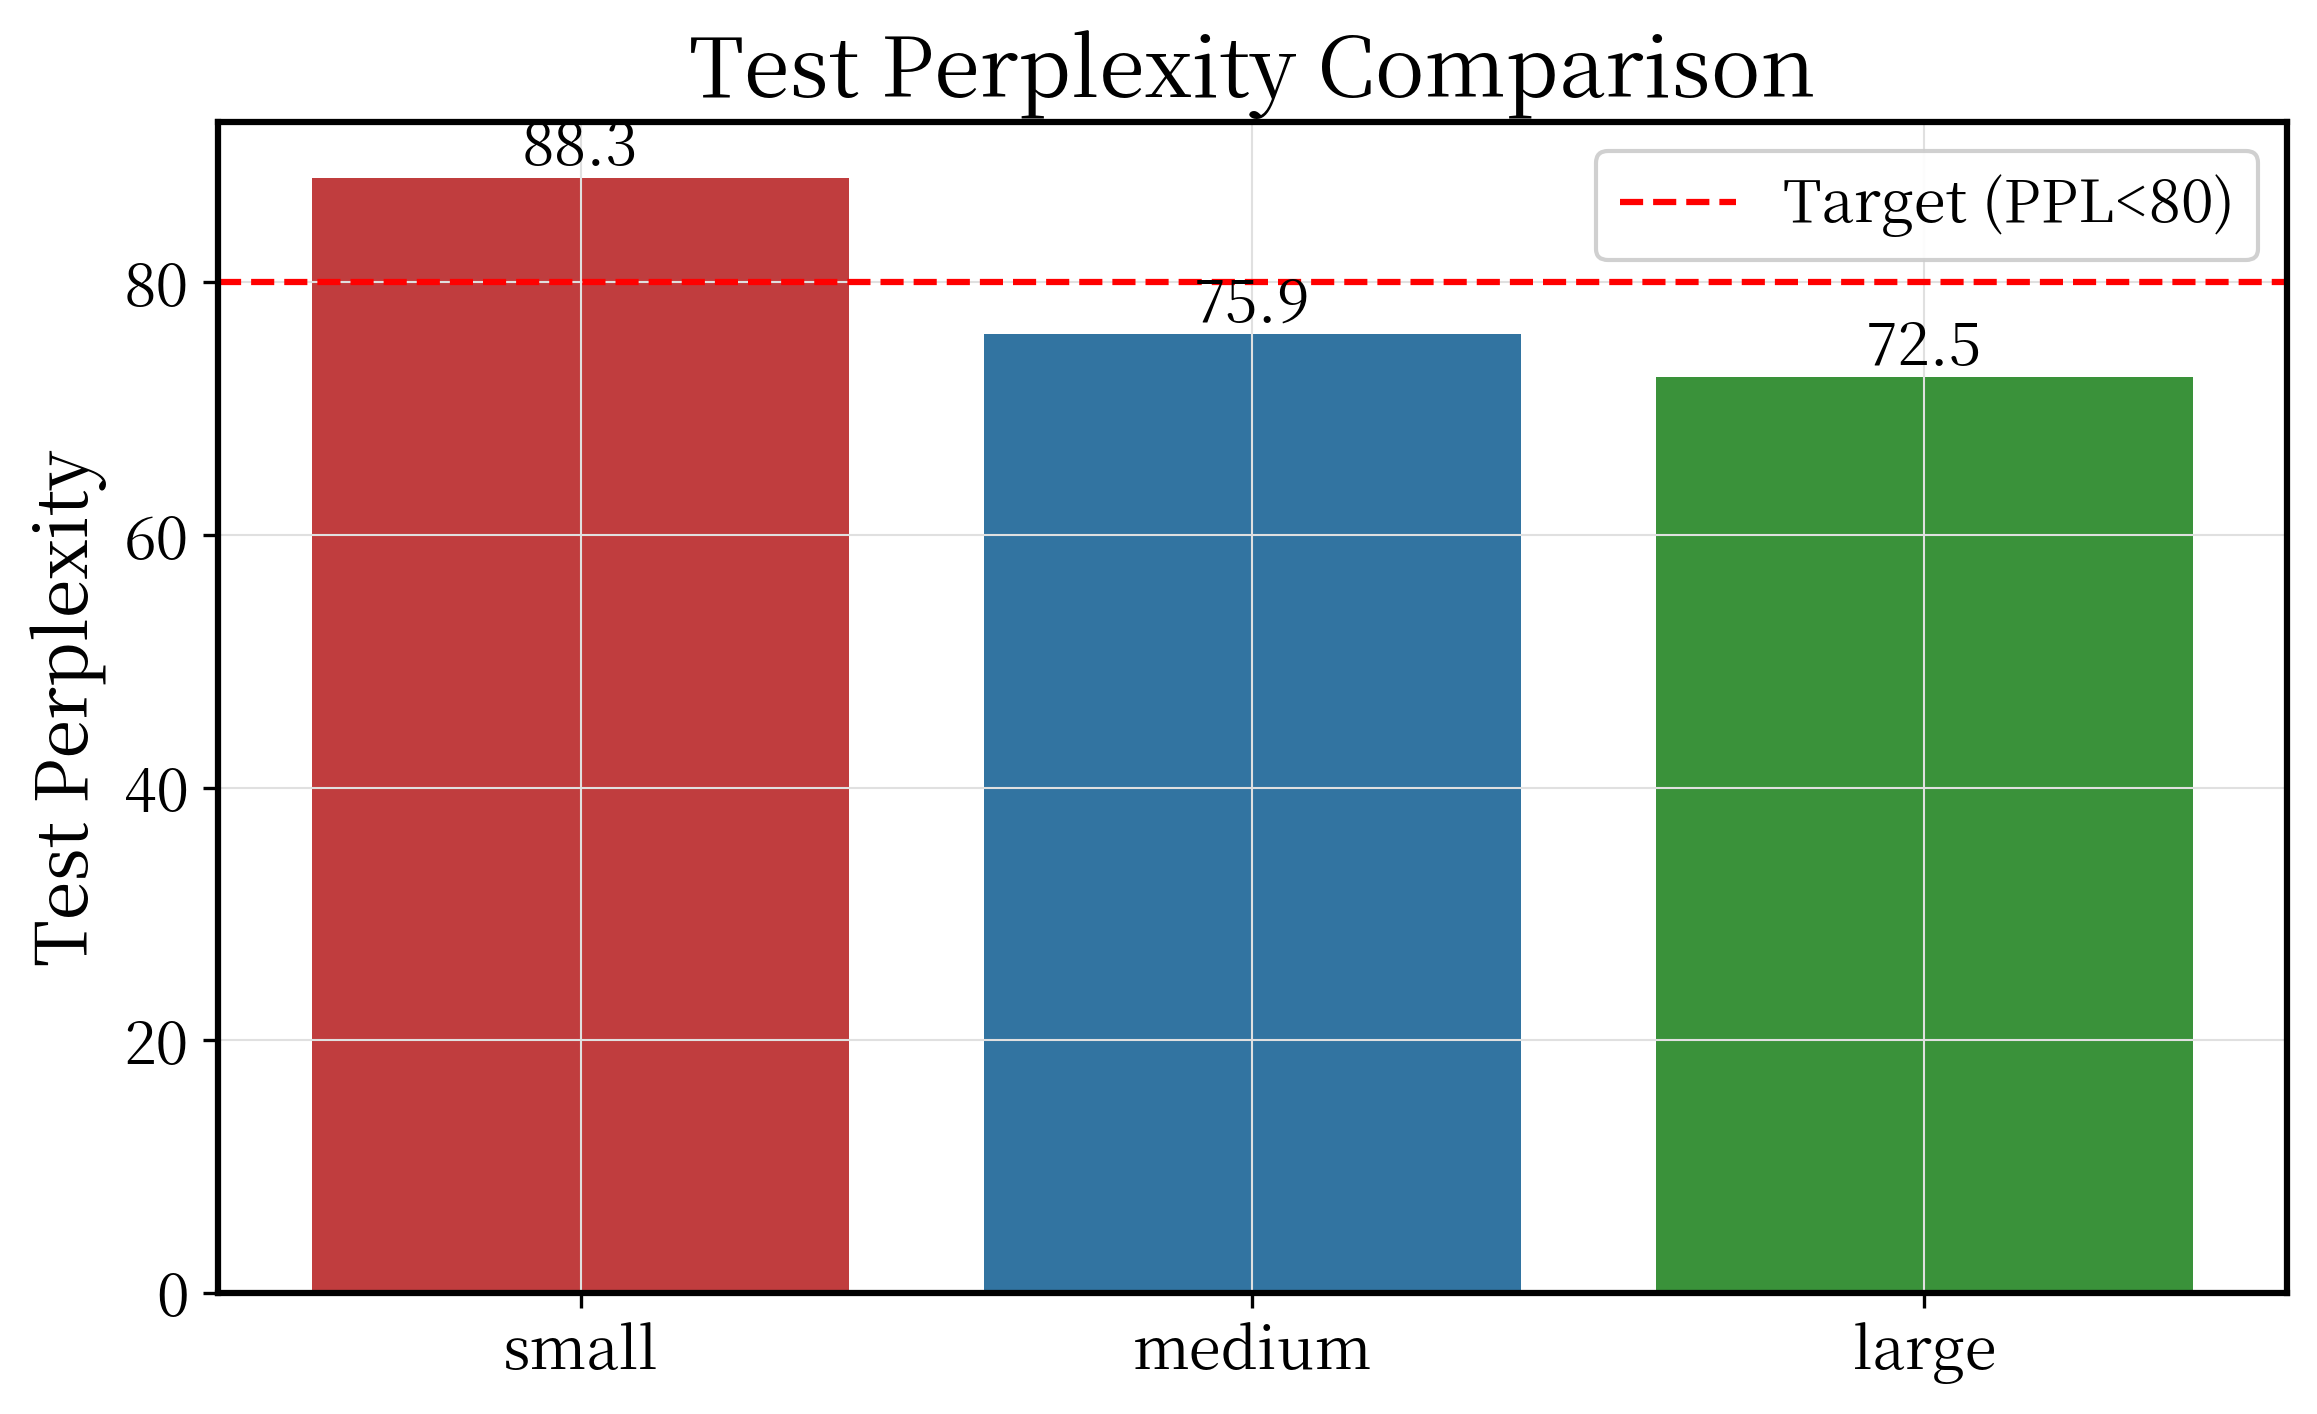
\includegraphics[width=0.8\textwidth]{figs/fig04_test_ppl.png}
\caption{测试集困惑度对比}
\label{fig:test_ppl}
\end{figure}

\subsection{训练效率分析}

图\ref{fig:time}记录了不同模型每轮训练的时间开销。Large模型每epoch约41.1秒，是Small模型（7.7秒）的5.3倍，但测试PPL仅从88.30降至72.48（改善18\%）。相比之下，Medium模型以2倍于Small的训练时间（15.5秒/epoch），将测试PPL从88.30降至75.92（改善14\%），在性价比上更为突出。

\begin{figure}[H]
\centering
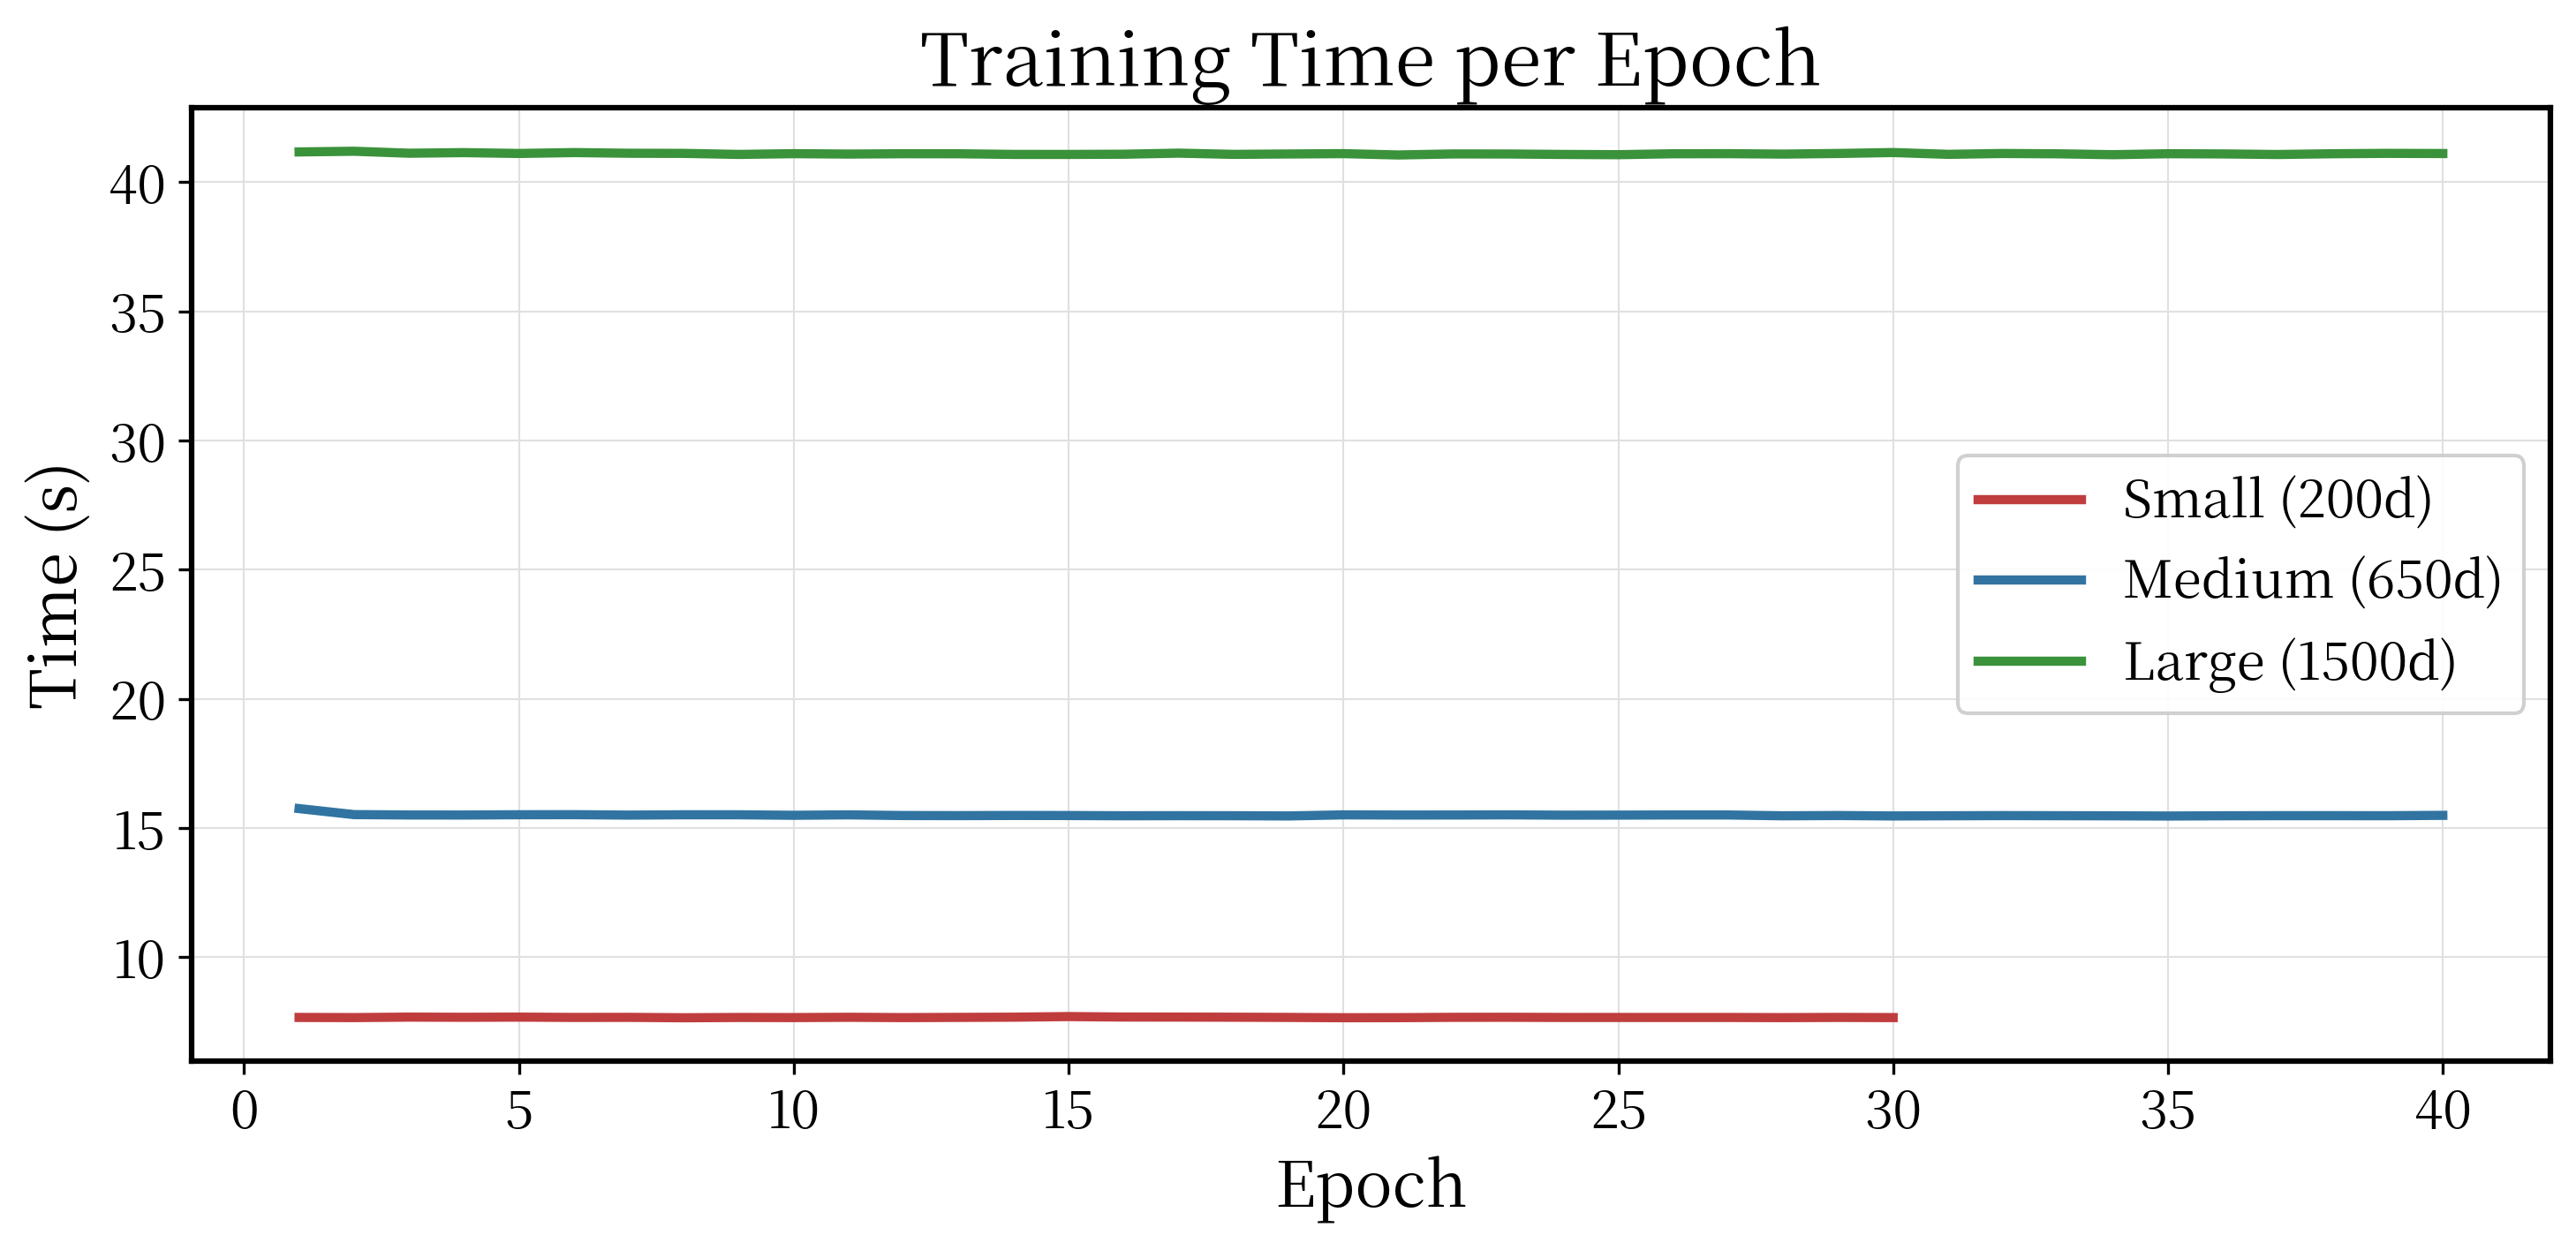
\includegraphics[width=0.8\textwidth]{figs/fig05_epoch_time.png}
\caption{每轮训练时间对比}
\label{fig:time}
\end{figure}

图\ref{fig:convergence}进一步分析了三种模型的收敛速度，以训练时间为横轴展示困惑度变化。可以看出Small模型虽然单epoch最快，但由于容量有限，其PPL改善很快饱和；Large模型每epoch较慢，但PPL的下降持续更久，最终在相同的总训练时间预算下，Large模型能达到更低的PPL。

\begin{figure}[H]
\centering
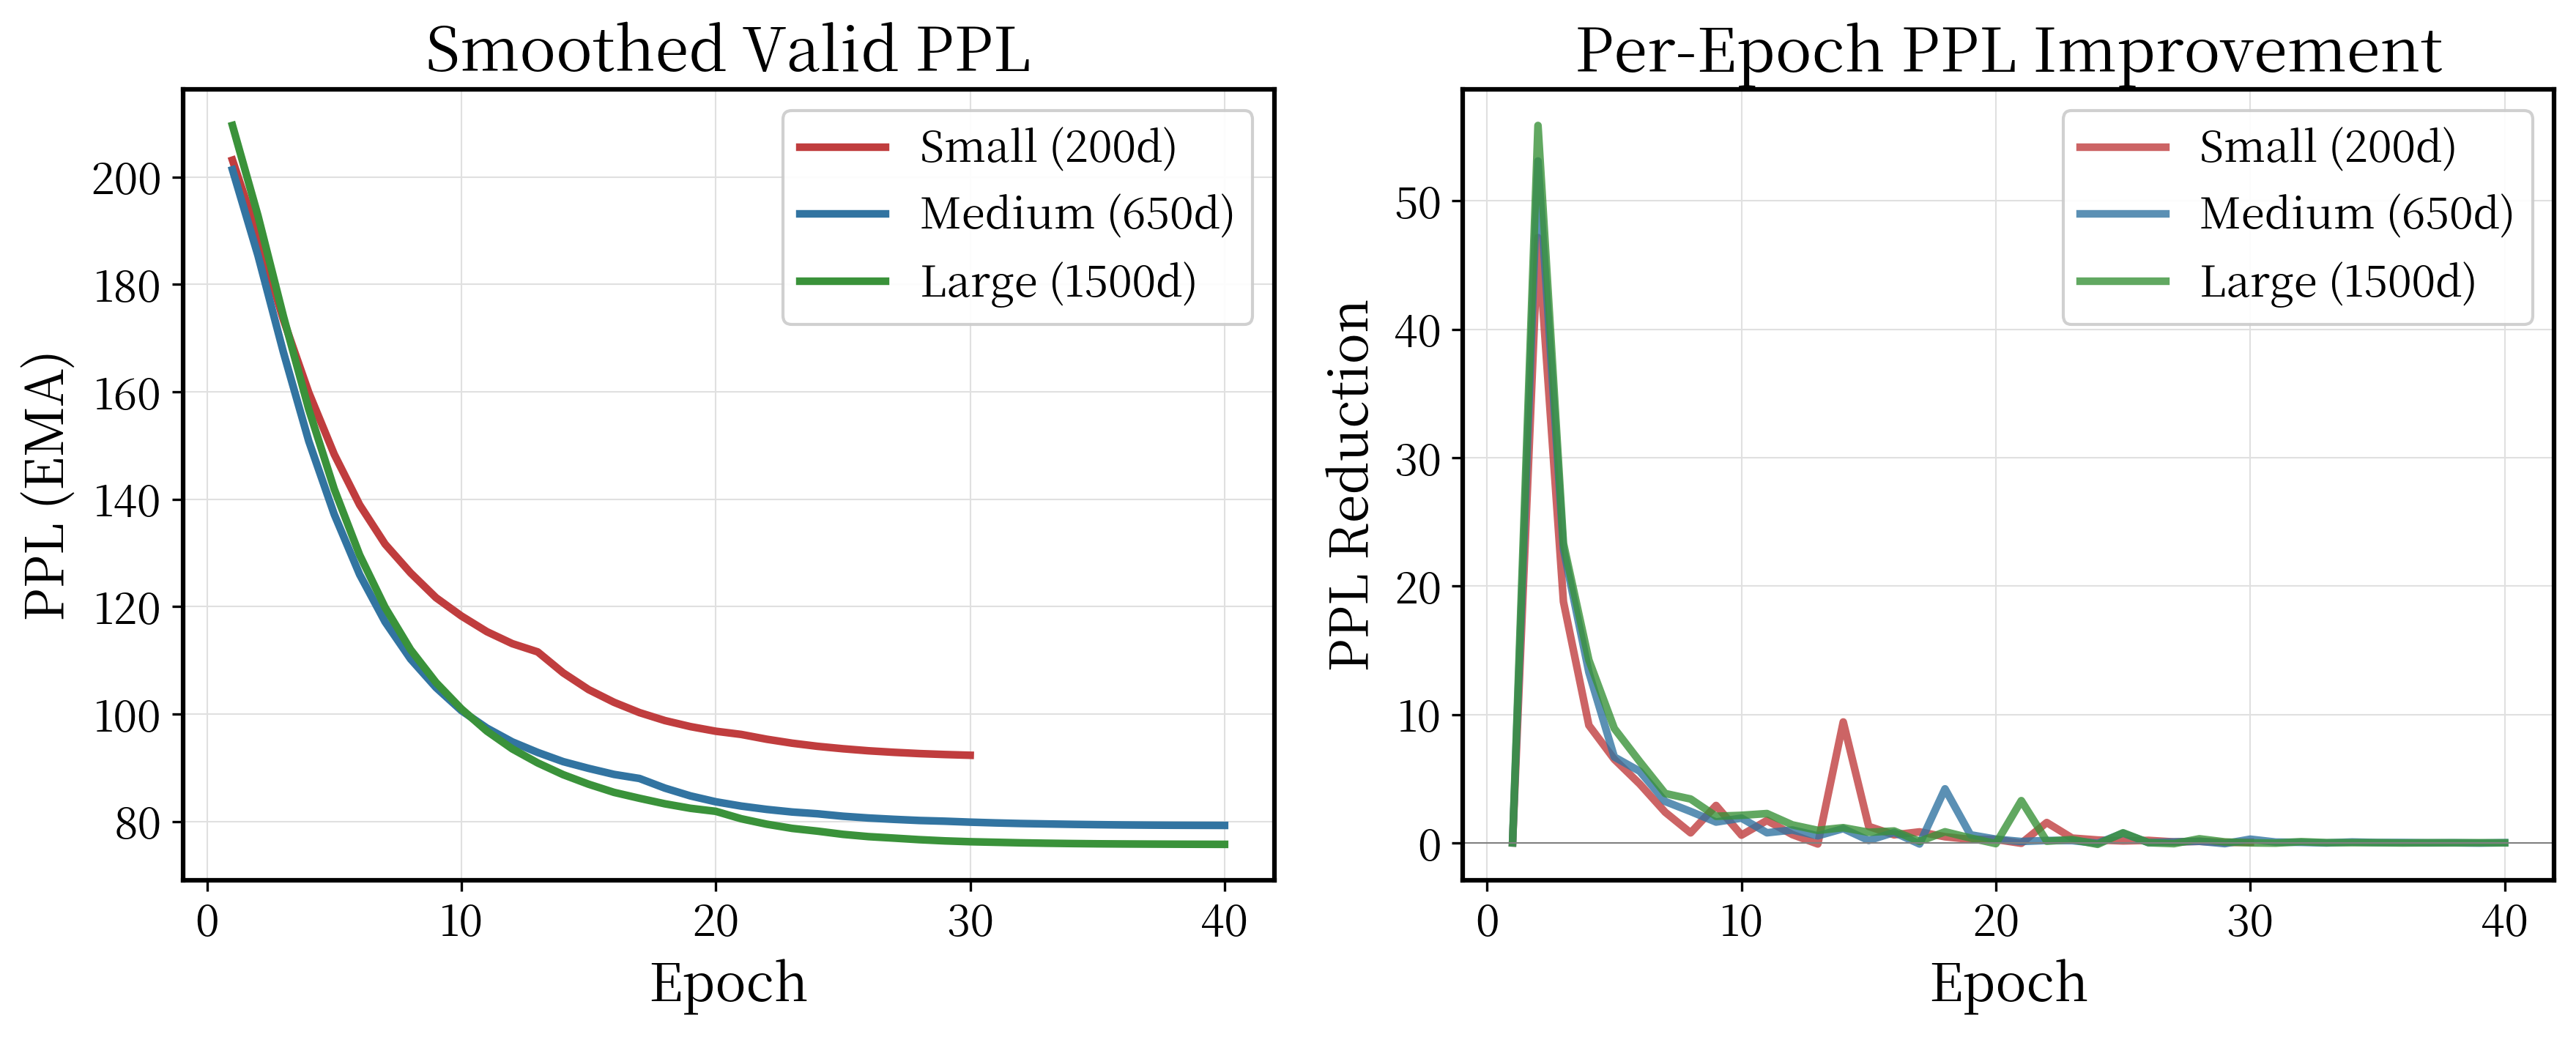
\includegraphics[width=0.8\textwidth]{figs/fig06_convergence.png}
\caption{收敛速度对比}
\label{fig:convergence}
\end{figure}

图\ref{fig:param}从参数效率角度对比三种模型。从Small到Medium，隐藏维度从200增加到650（3.25倍），测试PPL改善了14\%，这一阶段参数增加带来了显著的性能提升。从Medium到Large，隐藏维度从650增加到1500（2.3倍），测试PPL仅改善了4.5\%，体现了性能收益递减的规律。

\begin{figure}[H]
\centering
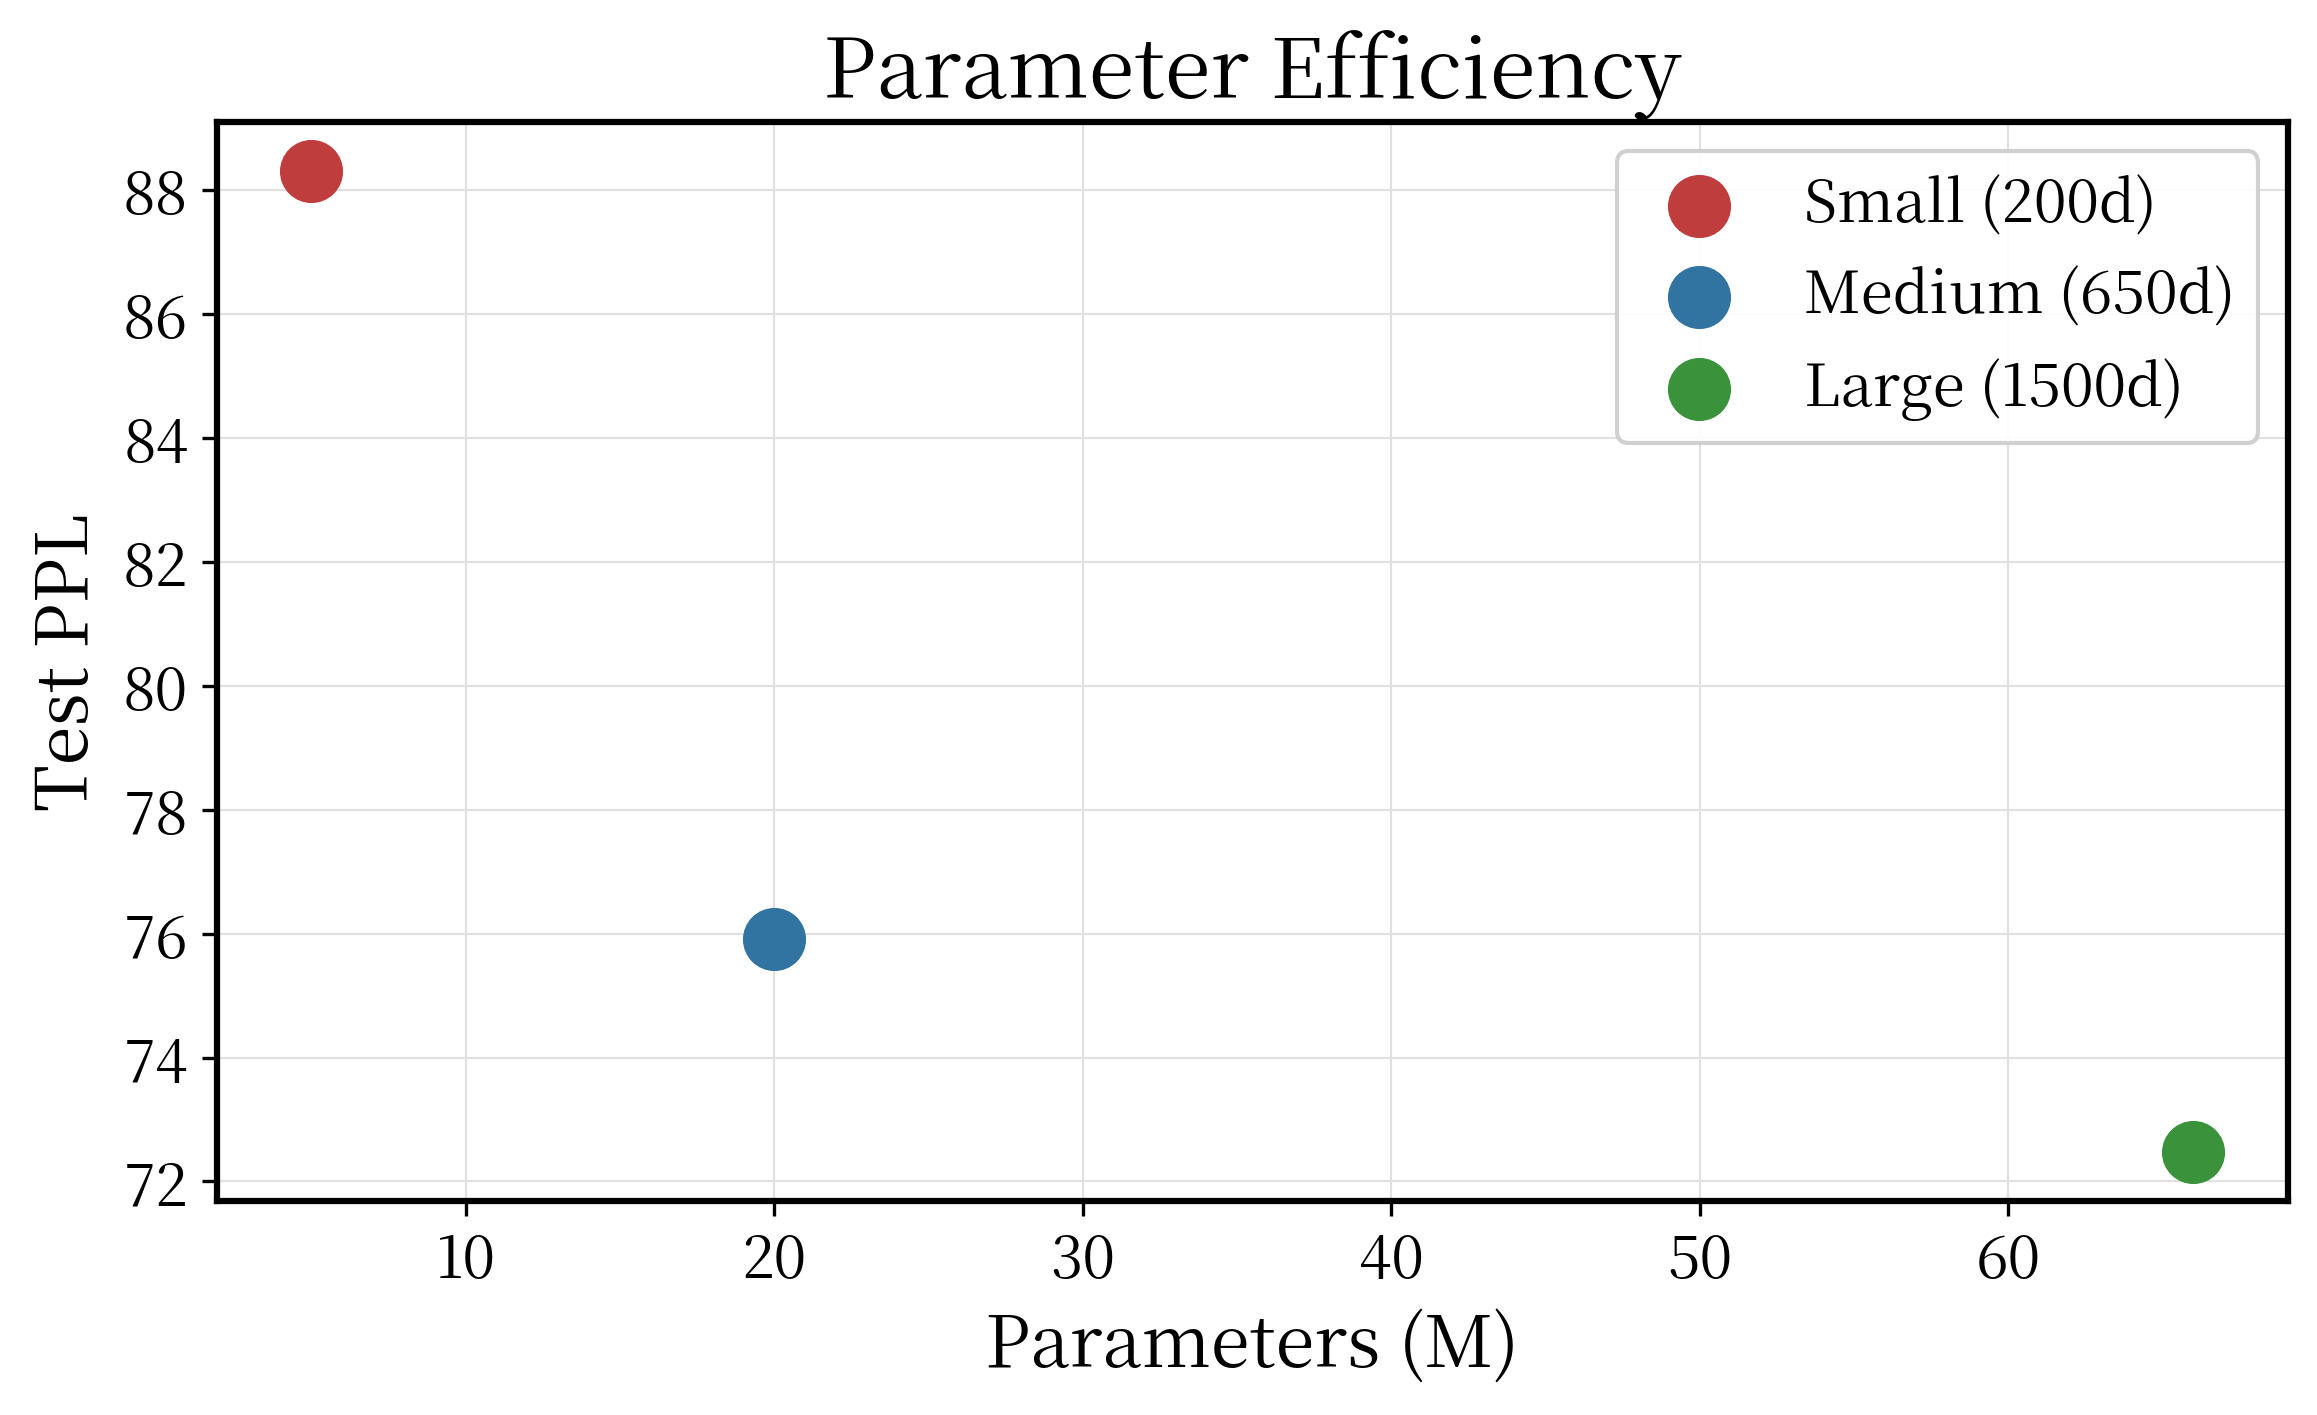
\includegraphics[width=0.8\textwidth]{figs/fig07_param_efficiency.png}
\caption{参数效率分析}
\label{fig:param}
\end{figure}

\section{深入讨论}

权重绑定是本实验中提升模型性能的关键技术之一。输入嵌入矩阵将词映射到连续向量空间，输出投影矩阵则将隐藏状态映射回词表空间，两者本质上都在建模词与语义向量之间的对应关系。共享这两个矩阵不仅减少了约三分之一的参数量（对于Large模型，词表10000$\times$隐藏1500的矩阵有15M参数，共享后节省可观），还通过参数共享的隐式正则化效果改善了泛化性能。

Dropout在LSTM语言模型中的应用需要特别注意：不能在时间步之间的循环连接上使用标准dropout，否则会破坏长期记忆的连续性。正确的做法是在层与层之间的垂直连接上应用dropout，或者采用变分dropout在整个序列上使用相同的dropout掩码。本实验中Dropout率随模型容量递增（0.2/0.5/0.65），实验结果表明这种匹配策略是有效的：Large模型在0.65 Dropout下仍能保持训练PPL=40.47和测试PPL=72.48之间合理的泛化差距。

从实验结果来看，模型容量的增大带来了性能收益递减的现象。Small到Medium的提升非常显著（测试PPL从88.30降至75.92，改善14\%），而Medium到Large的提升则相对有限（75.92降至72.48，改善4.5\%）。这表明PTB数据集929K训练词的规模限制了大型模型充分发挥其建模能力：Large模型的训练PPL（40.47）与测试PPL（72.48）之间的巨大差距（32 PPL）也说明，更大的模型主要在过拟合训练集，而非学到更深层的语言结构。在更大规模的语料上，大型模型的优势将更加明显。

\section{实验总结}

本实验成功实现了基于LSTM的神经网络语言模型，在Penn Treebank数据集上，Medium模型测试PPL=75.92、Large模型测试PPL=72.48，均达到了低于80的实验要求。通过对比三种不同规模的模型，深入理解了模型容量、正则化强度与泛化性能之间的平衡关系：容量过小（Small）导致欠拟合，容量增大带来的收益递减（Medium到Large仅改善4.5\%），而Dropout率需要与模型容量匹配递增。实验中掌握的权重绑定、层间Dropout、学习率衰减等技术对于后续的序列建模任务具有重要参考价值。

\begin{sloppypar}
本实验代码位于：\url{https://github.com/neverwinHao/deep-learning-project/tree/main/Exp7/code}
\end{sloppypar}

\end{document}
